\section{Experimental setup}
\label{sec:setup}

\begin{figure*}[t]
\centering
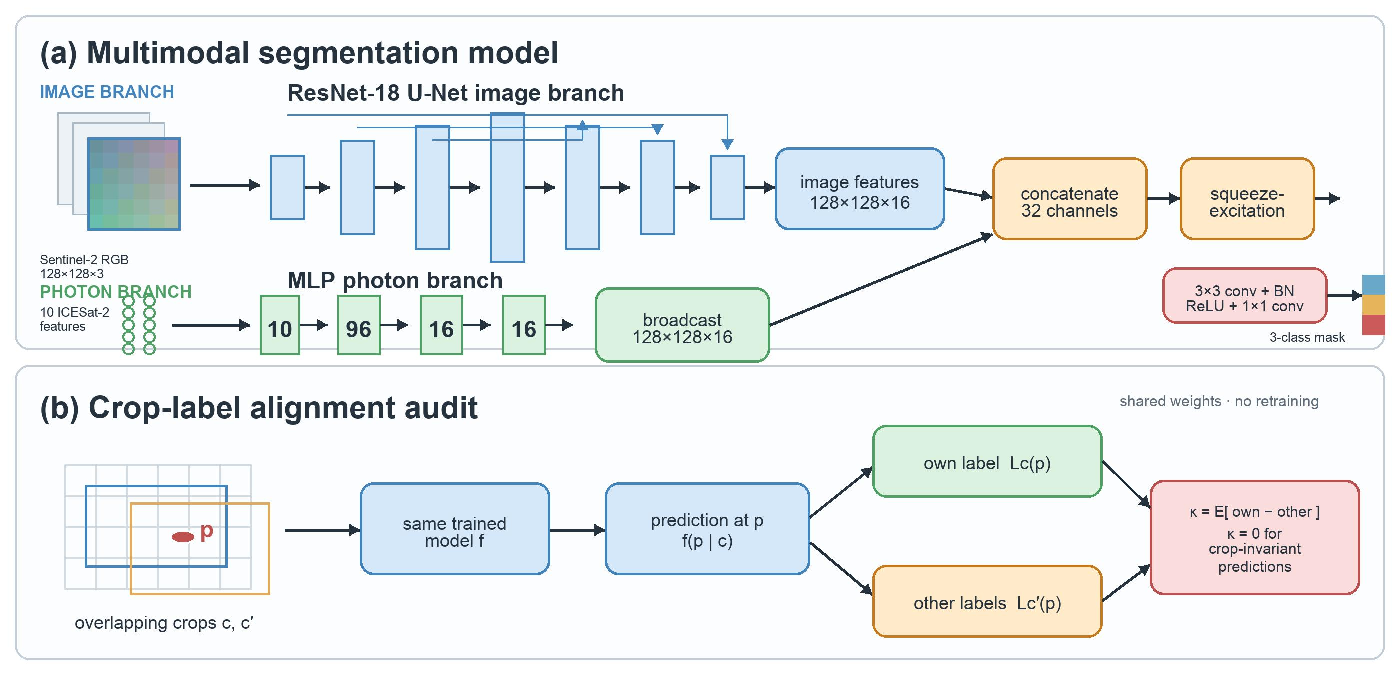
\includegraphics[width=0.72\textwidth]{figures/crop_alignment_architecture.pdf}
\caption{Model and audit schematic. The sea-ice model uses an ImageNet-initialized
ResNet-18 U-Net image branch and, in photon-enabled runs, an MLP branch for ICESat-2
features. The audit keeps weights fixed and compares agreement with the current
crop's label against other crops' labels for the same source pixel.}
\label{fig:architecture}
\end{figure*}

The supplement gives the full configuration. The sea-ice benchmark has 169{,}051
patches over 39 tiles and 17 acquisitions; the flood benchmark has 446 chips over 11
events, and the crop sweep draws 24 crops per chip per epoch from a $13 \times 13$
grid, evaluating $\kap$ on all 169 positions. The sea-ice model carries a second
branch that encodes ten co-registered ICESat-2 photon
features~\cite{neumann2019atlas} (\cref{fig:architecture}). The primary $\kap$ arm, at seed 42, disables that
branch and is optical-only. A seed-7 photon-enabled run is reported separately as an
input-mode sensitivity check, not averaged as a repeat seed.

Splits are leave-one-acquisition-out and leave-one-event-out, since that is the unit
sharing a labeller constant, and model selection never sees the held-out unit.
For crop-label alignment, both scorers retain every crop-read prediction and use
the source-pixel weighting, so each source pixel in the artefact set has equal
weight. Only the flood expert-label analysis mosaics hard predictions by majority
vote before scoring each source pixel once.

Training used two RTX A6000 cards capped at 300\,W; flood crop runs take about four
minutes each. Full optimisation settings are in the supplement.
